\documentclass[t,xcolor=dvipsnames]{beamer}

%%%%%%%%%%%%%%%%%%%%%%%% Packages/includes
\usepackage[english]{babel}
%\usepackage[latin1]{inputenc}
\usepackage{times}
\usepackage{pgfpages}
\usepackage{pgfplotstable}
\usepackage{booktabs}
\usepackage{subcaption}
\usepackage{epigraph}
% Antonio's macros
% !TEX root = thesis.tex
\definecolor{accolornotes}{rgb}{0.7,0.3,0.2}
\newcommand{\acnote}[1]{\textcolor{accolornotes}{[{\bf #1}]}}


\definecolor{jscolornotes}{rgb}{0.3,0.7,0.2}
\newcommand{\jsnote}[1]{\textcolor{jscolornotes}{[{\bf #1}]}}


\definecolor{acgray}{rgb}{0.8,0.8,0.8}
\newcommand{\acremove}[1]{\textcolor{acgray}{[{#1}]}}

\definecolor{myred}{rgb}{0.6, 0, 0}
\definecolor{myblue}{rgb}{0.3, 0.1, 0.9}

%\definecolor{acgreen}{rgb}{0.1,0.5,0.1}
%\definecolor{acblue}{rgb}{0.1,0.1,0.5}
%\newcommand{\bl}[1]{\textcolor{acgreen}{#1}}
%\newcommand{\gr}[1]{\textcolor{acblue}{#1}}

\newcommand{\eg}{{\it e.g.}\ }
\newcommand{\ie}{{\it i.e.}\ }
\newcommand{\vs}{{vs.}\ }
\newcommand{\etal}{{et al.}\ }
%\newcommand{\cf}{{\it cf}}

\newcommand{\be}{\begin{equation}}
\newcommand{\ee}{\end{equation}}
\newcommand{\bea}{\begin{eqnarray}}
\newcommand{\eea}{\end{eqnarray}}
\newcommand{\beas}{\begin{eqnarray*}}
\newcommand{\eeas}{\end{eqnarray*}}

\usepackage{tikz}

\newcommand{\circleplus}{ 
  \mathbin{
    \mathchoice
      {\buildcircleplus{\displaystyle}}
      {\buildcircleplus{\textstyle}}
      {\buildcircleplus{\scriptstyle}}
      {\buildcircleplus{\scriptscriptstyle}}
  } 
}

\newcommand\buildcircleplus[1]{%
  \begin{tikzpicture}[baseline=(X.base), inner sep=0, outer sep=0]
    \node[draw,circle] (X)  {$#1+$};
  \end{tikzpicture}%
}


\newcommand{\reflabel}{dummy} % Dummy initial reflabel - use renewcommand at the start of each chapter

%%%
%%% Stuff for vector typesetting  ----------------------------------------
%%%
%%%    e.g. use "\v a" or "\v r" for vectors
%%%
\def\vec#1{\mathchoice{\mbox{\boldmath  $\displaystyle\bf#1$}}
{\mbox{\boldmath  $\textstyle\bf#1$}}
{\mbox{\boldmath  $\scriptstyle\bf#1$}}
{\mbox{\boldmath  $\scriptscriptstyle\bf#1$}}}
\def\v#1{\protect\vec #1}

%%%
%%% Stuff for matrix typesetting  ----------------------------------------
%%%
%%%    e.g. use "\m M" or "\m A" for matrices
%%%
\def\mat#1{\mathchoice{\mbox{\boldmath$\displaystyle\tt#1$}}
{\mbox{\boldmath$\textstyle\tt#1$}}
{\mbox{\boldmath$\scriptstyle\tt#1$}}
{\mbox{\boldmath$\scriptscriptstyle\tt#1$}}}
\def\m#1{\protect\mat #1}

%%%
%%% Stuff for bold maths typesetting  ----------------------------------------
%%%
%%%   e.g. use "\bfmu" for boldface mu symbol
%%%
\def\bfmu{\mbox{\boldmath$\mu$}}
\def\bftau{\mbox{\boldmath$\tau$}}
\def\bftheta{\mbox{\boldmath$\theta$}}
\def\bfdelta{\mbox{\boldmath$\delta$}}
\def\bfphi{\mbox{\boldmath$\phi$}}
\def\bfpsi{\mbox{\boldmath$\psi$}}
\def\bfeta{\mbox{\boldmath$\eta$}}
\def\bfnabla{\mbox{\boldmath$\nabla$}}
\def\bfGamma{\mbox{\boldmath$\Gamma$}}

%%%
%%% Stuff for argmax argmin  ----------------------------------------
%%%
\DeclareMathOperator*{\argmax}{argmax}
\DeclareMathOperator*{\argmin}{argmin}


%%%
%%% Stuff for calligraphic style  ----------------------------------------
%%%
\DeclareMathAlphabet{\mathcal}{OMS}{cmsy}{m}{n}

%% code to highlight maximal/minimal entries in column tables with pgftables
\newcommand{\findmax}[3]{
    \pgfplotstablevertcat{\datatable}{#1}
    \pgfplotstablecreatecol[
    create col/expr={%
    \pgfplotstablerow
    }]{rownumber}\datatable
    \pgfplotstablesort[sort key={#2},sort cmp={float >}]{\sorted}{\datatable}%
    \pgfplotstablegetelem{0}{rownumber}\of{\sorted}%
    \pgfmathtruncatemacro#3{\pgfplotsretval}
    \pgfplotstableclear{\datatable}
}

\newcommand{\findmin}[3]{
    \pgfplotstablevertcat{\datatable}{#1}
    \pgfplotstablecreatecol[
      create col/expr={%
    \pgfplotstablerow
    }]{rownumber}\datatable
    \pgfplotstablesort[sort key={#2},sort cmp={float <}]{\sorted}{\datatable}%
    \pgfplotstablegetelem{0}{rownumber}\of{\sorted}%
    \pgfmathtruncatemacro#3{\pgfplotsretval}
    \pgfplotstableclear{\datatable}
}

\pgfplotstableset{
    highlight col max/.code 2 args={
        \findmax{#1}{#2}{\maxval}
        \edef\setstyles{\noexpand\pgfplotstableset{
                every row \maxval\noexpand\space column #2/.style={
                    postproc cell content/.append style={
                        /pgfplots/table/@cell content/.add={$\noexpand\bf}{$}
                    },
                }
            }
        }\setstyles
    },
    highlight col min/.code 2 args={
        \findmin{#1}{#2}{\minval}
        \edef\setstyles{\noexpand\pgfplotstableset{
                every row \minval\noexpand\space column #2/.style={
                    postproc cell content/.append style={
                        /pgfplots/table/@cell content/.add={$\noexpand\bf}{$}
                    },
                }
            }
        }\setstyles
    },
    highlight row max/.code 2 args={
        \pgfmathtruncatemacro\rowindex{#2-1}
        \pgfplotstabletranspose{\transposed}{#1}
        \findmax{\transposed}{\rowindex}{\maxval}
        \edef\setstyles{\noexpand\pgfplotstableset{
                every row \rowindex\space column \maxval\noexpand/.style={
                    postproc cell content/.append style={
                        /pgfplots/table/@cell content/.add={$\noexpand\bf}{$}
                    },
                }
            }
        }\setstyles
    },
    highlight row min/.code 2 args={
        \pgfmathtruncatemacro\rowindex{#2-1}
        \pgfplotstabletranspose{\transposed}{#1}
        \findmin{\transposed}{\rowindex}{\maxval}
        \edef\setstyles{\noexpand\pgfplotstableset{
                every row \rowindex\space column \maxval\noexpand/.style={
                    postproc cell content/.append style={
                        /pgfplots/table/@cell content/.add={$\noexpand\bf}{$}
                    },
                }
            }
        }\setstyles
    },
}

\makeatletter
\long\def\pgfplotstabletypeset@opt@collectarg[#1]#2{%

    \pgfplotstable@isloadedtable{#2}%
        {\pgfplotstabletypeset@opt@[#1]{#2}}%
        {\pgfplotstabletypesetfile@opt@[#1]{#2}}%
}
\makeatother


\usepackage{tikz}
\usetikzlibrary{arrows,positioning,matrix,scopes,calc,tikzmark,decorations.pathreplacing,shapes,decorations.markings,calc}
\tikzstyle{every picture}+=[remember picture]

%%%%%%%%%%%%%%%%%%%%%%%% Bibliography
\usepackage[backend=bibtex,style=authortitle]{biblatex}
\AtEveryCitekey{\iffootnote{\color{black}\tiny}{\color{black}}}
\addbibresource{../references.bib}

%%%%%%%%%%%%%%%%%%%%%%%% Beamer Mode

%\setbeameroption{hide notes}
%\setbeameroption{show notes}
%\setbeameroption{show notes on second screen=right}


%%%%%%%%%%%%%%%%%%%%%%%% Beamer Options/Settings

\mode<presentation>
{
  \usetheme{default}
  \setbeamercovered{transparent}
}

%\setbeamertemplate{note page}[plain]

% Get rid of the annoying symbol list
\beamertemplatenavigationsymbolsempty
% don't show bookmarks on initial view
\hypersetup{pdfpagemode=UseNone}

% Show page number in lower right
\setbeamertemplate{footline}{%
    \raisebox{5pt}{\makebox[\paperwidth]{\hfill\makebox[20pt]{\color{gray}
          \scriptsize\insertframenumber}}}\hspace*{5pt}}


\addtobeamertemplate{frametitle}{}{%
    \begin{tikzpicture}[remember picture,overlay]
    \node[anchor=north east,yshift=2pt] at (current page.north east) {
\includegraphics[height=1em]{uc-cmyk}};
    \end{tikzpicture}}

\definecolor{filtercolor}{RGB}{255,230,153}
\definecolor{filtershade}{RGB}{205,185,123}
\definecolor{fmcolor}{RGB}{231,230,230}
\definecolor{fmshade}{RGB}{186,185,185}

\setbeamercolor{title}{fg=White}
\setbeamercolor{author}{fg=White}
\setbeamercolor{institute}{fg=White}
\setbeamercolor{date}{fg=White}
%\setbeamercolor{section in head/foot}{fg=White}
%\setbeamercolor{author in head/foot}{fg=White}
%\setbeamercolor{date in head/foot}{fg=White}


%%%%%%%%%%%%%%%%%%%%%%%% Title Page Setup
\title[Conditional Computation and Restricted Connectivity in Deep Neural Networks] % (optional, use only with long paper titles)
{Conditional Computation and Restricted Connectivity in Deep Neural Networks}
%\subtitle
%{Improving CNN
%Generalization and
%Efficiency}

\author[Yani Ioannou]
{Yani Ioannou}

\institute[University of Cambridge] % (optional, but mostly needed)
{University of Cambridge}

\date{March 21, 2017}

%\pgfdeclareimage[height=0.5cm]{university-logo}{uc-cmyk}
%\logo{\pgfuseimage{university-logo}}

% Delete this, if you do not want the table of contents to pop up at
% the beginning of each subsection:
%\AtBeginSubsection[]
%{
%  \begin{frame}<beamer>{Outline}
%    \tableofcontents[currentsection,currentsubsection]
%  \end{frame}
%}

% If you wish to uncover everything in a step-wise fashion, uncomment
% the following command: 

%\beamerdefaultoverlayspecification{<+->}


\begin{document}

%%%%%%%%%%%%%%%%%%%% TITLE Frame

\usebackgroundtemplate{%             declare it
\tikz[overlay,remember picture] \node[opacity=0.95, at=(current page.center)] {
   \includegraphics[height=\paperheight,width=\paperwidth]{background}};
}

\begin{frame}
  \titlepage
\end{frame}


\usebackgroundtemplate{%             declare it
\tikz[overlay,remember picture] \node[opacity=0.2, at=(current page.center)] {
   \includegraphics[height=\paperheight,width=\paperwidth]{background}};
}

%\begin{frame}{Outline}
%  \tableofcontents
  % You might wish to add the option [pausesections]
%\end{frame}


% Since this a solution template for a generic talk, very little can
% be said about how it should be structured. However, the talk length
% of between 15min and 45min and the theme suggest that you stick to
% the following rules:  

% - Exactly two or three sections (other than the summary).
% - At *most* three subsections per section.
% - Talk about 30s to 2min per frame. So there should be between about
%   15 and 30 frames, all told.

\section{Introduction}
\begin{frame}{About Me}
\begin{itemize}
\item Ph.D.\ student in the Department of Engineering at the University of Cambridge.
%\item Funded by a Microsoft Research PhD Scholarship
\item Supervised by Professor Roberto Cipolla, head of the Computer Vision and Robotics group in the Machine Intelligence Lab, and Dr. Antonio Criminisi, a principal researcher at Microsoft Research.
\end{itemize}
\centering
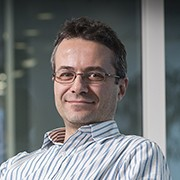
\includegraphics[width=0.207\linewidth]{antonio}~
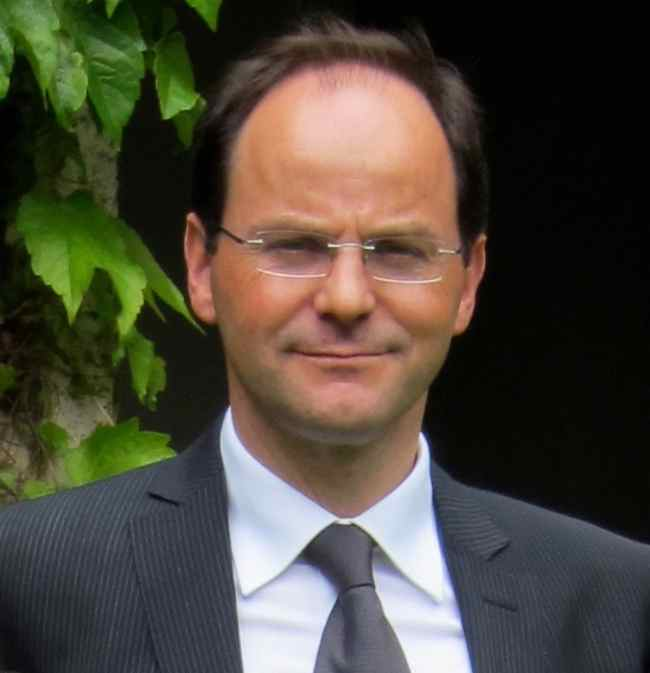
\includegraphics[width=0.2\linewidth]{roberto}
\end{frame}

\usebackgroundtemplate{}

\section{Areas of Research}
\begin{frame}{Collaborative Research @ MSR}
\begin{itemize}
    \item Segmentation of brain tumor tissues with convolutional neural networks.\\{\footnotesize D.\ Zikic, Y.\ Ioannou, M.\ Brown, A.\ Criminisi.\\MICCAI-BRATS 2014}
    \item Measuring Neural Net Robustness with Constraints.\\{\footnotesize O.\ Bastani, Y.\ Ioannou, L.\ Lampropoulos, D\ Vytiniotis, A.\ Nori, A.\ Criminisi.\\NIPS 2016}
    \item Refining Architectures of Deep Convolutional Neural Networks.\\{\footnotesize 
S.\ Shankar, D.\ Robertson, Y.\ Ioannou, A.\ Criminisi, R.\ Cipolla.\\CVPR 2016}
\end{itemize}
\end{frame}

\begin{frame}{Collaborative Research @ MSR}
\textbf{Segmentation of brain tumor tissues with convolutional neural networks.}\\{\footnotesize D.\ Zikic, Y.\ Ioannou, M.\ Brown, A.\ Criminisi.\\MICCAI-BRATS 2014}
\begin{itemize}
    \item One of the first papers using deep learning for volumetric/medical imagery
    \item Biggest challenge for training was the class-imbalanced training data
\end{itemize}
\end{frame}

\begin{frame}{Collaborative Research @ MSR}
\textbf{Measuring Neural Net Robustness with Constraints.}\\{\footnotesize O.\ Bastani, Y.\ Ioannou, L.\ Lampropoulos, D\ Vytiniotis, A.\ Nori, A.\ Criminisi.\\NIPS 2016}
\begin{itemize}
    \item Showed that contemporary methods of finding adversarial examples were limited in their coverage
    \item Found that not all adversarial images can be used to improve network robustness
\end{itemize}
\end{frame}

\begin{frame}{Collaborative Research @ MSR}
\textbf{Refining Architectures of Deep Convolutional Neural Networks.}\\{\footnotesize S.\ Shankar, D.\ Robertson, Y.\ Ioannou, A.\ Criminisi, R.\ Cipolla.\\CVPR 2016}
\begin{itemize}
    \item A method for adapting network architectures optimized for large datasets for smaller datasets
    \item Attempts to answer the common problem of adapting contemporary research to real-world problems
\end{itemize}
\end{frame}

\begin{frame}{First Author Publications during PhD}
\begin{itemize}
    \item Decision Forests, Convolutional Networks and the Models in-Between.\\{\footnotesize Y.\ Ioannou, D.\ Robertson, D.\ Zikic, P.\ Kontschieder, J.\ Shotton, M.\ Brown, A.\ Criminisi.\\MSR Technical Report} 
    \item Training CNNs with Low-Rank Filters for Efficient Image Classification.\\{\footnotesize Y.\ Ioannou, D.\ Robertson, J.\ Shotton, R.\ Cipolla, A.\ Criminisi. \\ICLR 2016}
    \item Deep roots: Improving CNN efficiency with hierarchical filter groups.\\{\footnotesize Y.\ Ioannou, D.\ Robertson, R.\ Cipolla, A.\ Criminisi.\\CVPR 2017}
    
\end{itemize}
\end{frame}
\section{Motivation}

%%%%%%%%%%%%%%%%%%%%

\begin{frame}{ILSVRC}{Imagenet Large-Scale Visual Recognition Challenge}

\begin{figure}
    
\includegraphics[width=0.4\textwidth]{imagenetlogo}
\end{figure}
\begin{itemize}
    \item Imagenet Large-Scale Visual Recognition Challenge.
    \item 1.2 Million Training Images, 1000 classes.
    \item 50,000 image validiation/test set.
    \begin{itemize}
        \item In 2012 Alex Krizhevsky won challenge with CNN.
        \item `Alexnet' was 26.2\% better than second best, 15.3\%.
    \end{itemize}
    \item State-of-the-art beats human error (5\%).
\end{itemize}    
\end{frame}

%%%%%%%%%%%%%%%%%%%%

\begin{frame}{AlexNet Complexity}
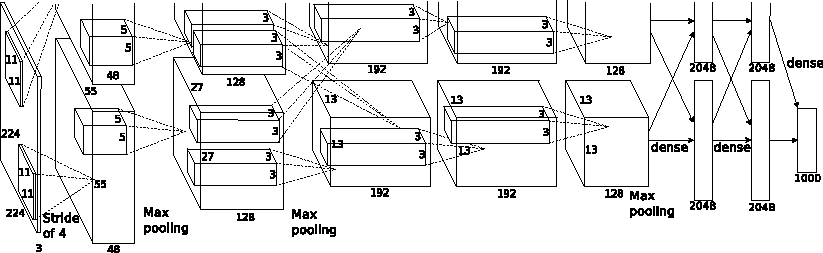
\includegraphics[width=\columnwidth]{alexnet}
\begin{itemize}
\item $\approx$ 61 million parameters %60,965,224
\item $\approx$ 724 million FLOPS (per-sample) % 724,417,384
\item Imagenet has 1.28 million training samples ($227 \times 227 \times 3$) %227×227×3×1281167
\item Images of dimensions  ($227 \times 227 \times 3$) $\approx$ 200 billion pixels % %227×227×3×1281167 = 198,051,763,029
\end{itemize}
\end{frame}

\begin{frame}{AlexNet Complexity - FLOPS}
\centering
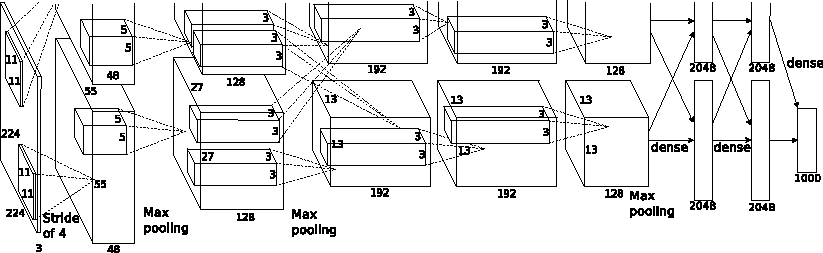
\includegraphics[width=0.9\columnwidth]{alexnet}
\tikzstyle{every node}=[font=\tiny]
\pgfplotstableread[col sep=comma]{alexnetma.csv}\datatable
\begin{tikzpicture}
\begin{axis}[
    axis x line=bottom,
    axis y line=left,
    ybar=0pt,
    bar width=1em,
    width=\linewidth,
    height=0.4\linewidth,
    enlarge x limits=0.1,
    ylabel=FLOPS,
    y label style={at={(axis description cs:0.09,.5)},anchor=south},
    y tick label style={
        /pgf/number format/.cd,
            fixed,
            fixed zerofill,
            precision=1,
        /tikz/.cd
    },
    ymin=0,
    xticklabels from table={\datatable}{layer},
    xticklabel style = {rotate = 90, xshift = -0.8ex, anchor = mid east, font=\tiny},
    xtick=data,
]
\addplot[ybar, draw=none, fill=red!40] table [x expr=\coordindex,y=ma]{\datatable};
\end{axis}
\end{tikzpicture}
\end{frame}

\begin{frame}{AlexNet Complexity - Parameters}
\centering
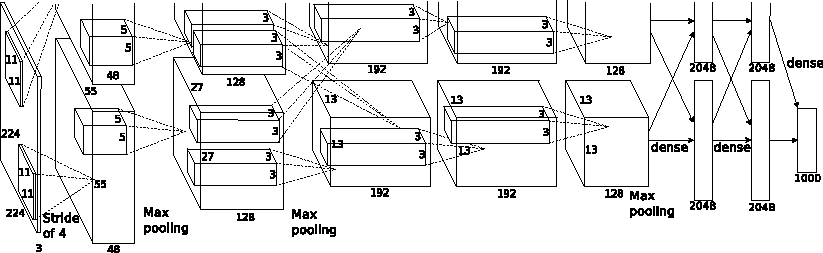
\includegraphics[width=0.9\columnwidth]{alexnet}
\tikzstyle{every node}=[font=\tiny]
\pgfplotstableread[col sep=comma]{alexnetma.csv}\datatable
\begin{tikzpicture}
\begin{axis}[
    axis x line=bottom,
    axis y line=left,
    ybar=0pt,
    bar width=1em,
    width=\linewidth,
    height=0.4\linewidth,
    enlarge x limits=0.1,
    ylabel=Parameters,
    y label style={at={(axis description cs:0.09,.5)},anchor=south},
    y tick label style={
        /pgf/number format/.cd,
            fixed,
            fixed zerofill,
            precision=1,
        /tikz/.cd
    },
    ymin=0,
    xticklabels from table={\datatable}{layer},
    xticklabel style = {rotate = 90, xshift = -0.8ex, anchor = mid east, font=\tiny},
    xtick=data,
]
\addplot[ybar, draw=none, fill=red!40] table [x expr=\coordindex,y=param]{\datatable};
\end{axis}
\end{tikzpicture}
$\approx$ 96\% in fully connected layers
%0.961714567
%0.038285433
\end{frame}

%%%%%%%%%%%%%%%%%%%%
\begin{frame}{AlexNet Complexity}
\begin{figure}[tbp]
\centering
\tikzstyle{every node}=[font=\tiny]
\pgfplotstableread[col sep=comma]{alexnetma.csv}\datatable
\begin{tikzpicture}
\begin{axis}[
    axis x line=bottom,
    axis y line=left,
    ybar=0pt,
    bar width=1em,
    width=0.9\linewidth,
    height=0.33\linewidth,
    enlarge x limits=0.1,
    ylabel=FLOPS,
    y label style={at={(axis description cs:0.09,.5)},anchor=south},
    y tick label style={
        /pgf/number format/.cd,
            fixed,
            fixed zerofill,
            precision=1,
        /tikz/.cd
    },
    ymin=0,
    xmajorticks=false,
    legend style={at={(0.5,1.2)},
    draw=none, anchor=north,legend columns=-1},
    area legend,
]
\addplot[ybar, draw=none, fill=red!40] table [x expr=\coordindex,y=ma]{\datatable};
\end{axis}
\end{tikzpicture}
~
\begin{tikzpicture}
\begin{axis}[
    axis x line=bottom,
    axis y line=left,
    ybar=0pt,
    bar width=1em,
    width=0.9\linewidth,
    height=0.33\linewidth,
    enlarge x limits=0.1,
    ylabel=Parameters,
    y label style={at={(axis description cs:0.09,.5)},anchor=south},
    y tick label style={
        /pgf/number format/.cd,
            fixed,
            fixed zerofill,
            precision=1,
        /tikz/.cd
    },
    ymin=0,
    xticklabels from table={\datatable}{layer},
    xticklabel style = {rotate = 90, xshift = -0.8ex, anchor = mid east, font=\tiny},
    xtick=data,
]
\addplot[ybar, draw=none, fill=red!40] table [x expr=\coordindex,y=param]{\datatable};
\end{axis}
\end{tikzpicture}
\end{figure}
\end{frame}
%%%%%%%%%%%%%%%%%%%%
\begin{frame}{Contemporary Complexity}
TODO: show graph of contemporary model complexity
\end{frame}

%%%%%%%%%%%%%%%%%%%%
\begin{frame}{Hinton Philosophy}
% http://sms.cam.ac.uk/media/2017973?format=mpeg4&quality=720p
    %\item Standard practice: Create a model of appropriate size for our data and the problem at hand.
    %\item Hinton philosophy on neural network design: Create a massively overparameterized network, and regularize like crazy to prevent overfitting.
    %\item Why is the latter needed in practice?
    %\item ``If you give me any sized dataset, what you ought to do if you want good generalization is get yourself into the small data regime. That is, however big your dataset, you ought to make a much bigger model so that that's small data. So, I think what the brain is doing is making sure that big data is small data and then regularizing the hell out of it, and that's a better thing to do than what statisticians used to think you should do, which is have a small model. And you can think of it as, it's just and efficient way of averaging many, many small models, which is a good way to use argback??, but something a bit more efficient than just doing a normal ensemble. So you should always, if you can, be in the small data regime by having a really big computer. And that's certainly where we live, because we have a limited lifetime so the amount of data we get is limited.''

\begin{quote}
``If you give me any sized dataset, what you ought to do \textbf{if you want good generalization} is get yourself into the small data regime. That is, however big your dataset, you ought to \textbf{make a much bigger model} so that that's small data.''\\

``So, I think what the brain is doing is \ldots \textbf{regularizing the hell} out of it, and that's a better thing to do than what statisticians used to think you should do, which is have a small model.'' \\
\flushright{\normalfont Geoffery Hinton\\Cambridge, June 2015}
\end{quote}
\end{frame}

%%%%%%%%%%%%%%%%%%%%
\begin{frame}{Hinton Philosophy}
% http://sms.cam.ac.uk/media/2017973?format=mpeg4&quality=720p
\begin{itemize}
    \item Hinton philosophy on neural network design: Create a massively over-parameterized network, and ``regularize like hell'' to prevent over-fitting.
    \item This seems to work well in practice for networks such as AlexNet, VGG, and MSRA
    \item But there is something that feels fundamentally wrong about this (and I'm not a statistician!)
    \item This feeling is backed up not only by my work, but by recent work showing that regularization in deep networks is not as effective as the community thought.
\end{itemize}
\end{frame}

%%%%%%%%%%%%%%%%%%%%
\begin{frame}{Alternative Philosophy}
\begin{itemize}
    \item Deep networks need many more parameters than data points because they aren't just learning to model data, but also learning what \emph{not} to learn. 
    %\begin{itemize}
    %    \item Isn't this what regularization is for? Yes, but it's more like using a sledgehammer on a small nail.
    %\end{itemize}
    % Sort of like regularization, but regularization is like using a sledge hammer on a nail, it affect a lot more than what you want
    \item Idea: Why don't we tell the network, through structural priors, not to learn things it doesn't need to?
    %\item Let's separate learning into two distinct functions:
    %\begin{itemize}
    %    \item Learning weights such that a filter responds to a stimulus
    %    \item Learning what to ignore
    %\end{itemize}
    \item Best example of this idea is a CNN!
    \begin{itemize}
        \item Shared parameters: filter learned for one part of the image should apply to the whole image.
        \item Filters: natural images are highly correlated locally
    \end{itemize}
    %\item A fully-connected network could theoretically learn the same thing, but in practice it never will.
\end{itemize}
\end{frame}
%%%%%%%%%%%%%%%%%%%%

TODO - INSERT LOW RANK STUFF HERE

%%%%%%%%%%%%%%%%%%%%

\begin{frame}{Typical Convolutional Layer}
\begin{figure}
   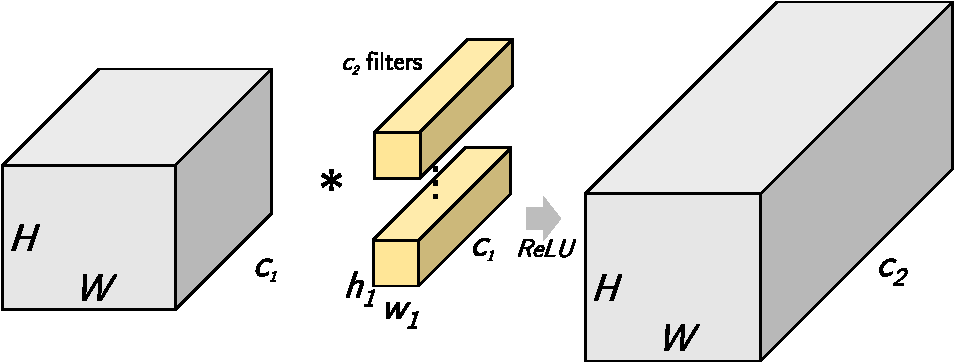
\includegraphics[width=0.9\textwidth, page=1]{../Figs/PDF/groupfig}
%   \caption{A full rank convolutional layer.}
\end{figure}
\begin{figure}

   \resizebox {0.5\textwidth} {!} {
   \begin{tikzpicture}[
       decoration={
          markings,
          mark=at position 1 with {\arrow[scale=2,gray]{latex}};
        }]
        % draw featuremap
        \pgfmathsetmacro{\cubex}{2}
        \pgfmathsetmacro{\cubey}{2}
        \pgfmathsetmacro{\cubez}{1.5}
        \draw[black,fill=fmcolor] (0,0,0) -- ++(-\cubex,0,0) -- ++(0,-\cubey,0) -- ++(\cubex,0,0) -- cycle;
        \draw[black,fill=fmshade] (0,0,0) -- ++(0,0,-\cubez) -- ++(0,-\cubey,0) -- ++(0,0,\cubez) -- cycle;
        \draw[black,fill=fmcolor] (0,0,0) -- ++(-\cubex,0,0) -- ++(0,0,-\cubez) -- ++(\cubex,0,0) -- cycle;
        \draw (-0.7, -2.5) node {image/feature map};
        
        \draw (1, -0.7) node {\LARGE$*$};
        
        % draw filter
        \pgfmathsetmacro{\cubex}{0.3}
        \pgfmathsetmacro{\cubey}{0.3}
        \pgfmathsetmacro{\cubez}{1.5}
        \draw[black,fill=filtercolor] (2,-0.7,0) -- ++(-\cubex,0,0) -- ++(0,-\cubey,0) -- ++(\cubex,0,0) -- cycle;
        \draw[black,fill=filtershade] (2,-0.7,0) -- ++(0,0,-\cubez) -- ++(0,-\cubey,0) -- ++(0,0,\cubez) -- cycle;
        \draw[black,fill=filtercolor] (2,-0.7,0) -- ++(-\cubex,0,0) -- ++(0,0,-\cubez) -- ++(\cubex,0,0) -- cycle;
        \draw (2.2, -2.5) node {filter};
            
        % draw output featuremap
        \pgfmathsetmacro{\cubex}{2}
        \pgfmathsetmacro{\cubey}{2}
        \pgfmathsetmacro{\cubez}{0.1}
        \draw[black,fill=fmcolor] (6,0,-0.75) -- ++(-\cubex,0,0) -- ++(0,-\cubey,0) -- ++(\cubex,0,0) -- cycle;
        \draw[black,fill=fmshade] (6,0,-0.75) -- ++(0,0,-\cubez) -- ++(0,-\cubey,0) -- ++(0,0,\cubez) -- cycle;
        \draw[black,fill=fmcolor] (6,0,-0.75) -- ++(-\cubex,0,0) -- ++(0,0,-\cubez) -- ++(\cubex,0,0) -- cycle;
        \draw (-0.7, -2.5) node {image/feature map};
        
        \draw[gray,postaction={decorate}] (2.7,-0.7) -- (3.8, -0.7);
        
        \draw (5.2, -2.5) node {output featuremap};
    \end{tikzpicture}
    }
\end{figure}
    \note[item]{We show here a typical convolutional layer.}
    \note[item]{Yellow blocks are filters.}
    \note[item]{Grey blocks are images or feature maps.}
\end{frame}

%%%%%%%%%%%%%%%%%%%
\begin{frame}{AlexNet Filter Grouping}
\begin{figure}
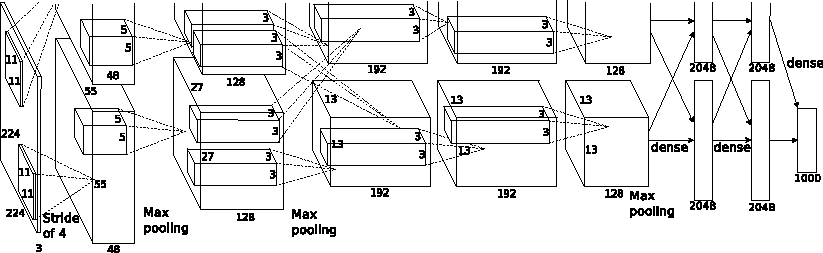
\includegraphics[width=\columnwidth]{alexnet}
\end{figure}
\begin{itemize}
\item Uses 2 filter groups in most of the convolutional layers
\item Allowed training across two GPUs (model parallelism)
\end{itemize}
\end{frame}

%%%%%%%%%%%%%%%%%%%

\begin{frame}{AlexNet Filter Grouping}
	\centering
    \begin{figure}
    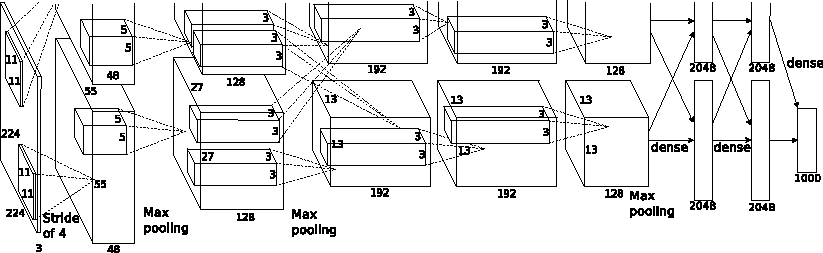
\includegraphics[width=0.9\columnwidth]{alexnet}
    \end{figure}
	\pgfplotstableread[col sep=comma]{../rootdata/alexnetma.csv}\datatable
	\pgfplotsset{major grid style={dotted,red}}
	
	\begin{tikzpicture}
	\begin{axis}[
	width=\linewidth,
	height=0.4\linewidth,
	axis x line=bottom,
	ylabel=Top-5 Val.\ Error,
	xlabel=Model Parameters (\# floats),
	axis lines=left,
	enlarge x limits=0.12,
	enlarge y limits=0.1,
	grid=major,
	%xmin=0,
	ytick={0.01,0.02,...,0.21},
	ymin=0.18,ymax=0.2,
	yticklabel={\pgfmathparse{\tick*100}\pgfmathprintnumber{\pgfmathresult}\%},style={
		/pgf/number format/fixed,
		/pgf/number format/precision=1
	},
	legend style={at={(0.98,0.98)}, anchor=north east, column sep=0.5em},
	legend columns=2,
	]
	\addplot[mark=*,mark options={fill=black},nodes near coords,only marks,
	point meta=explicit symbolic,
	] table[meta=Network,x=Param.,y expr={1 - \thisrow{Top-5 Acc.} },]{\datatable};
	\end{axis}
	\end{tikzpicture}
	\end{frame}

%%%%%%%%%%%%%%%%%%%%

\begin{frame}{Grouped Convolutional Layer}
\begin{figure}
   \includegraphics[width=0.9\textwidth, page=2]{../Figs/PDF/groupfig}
%   \caption{A full rank convolutional layer.}
\end{figure}
\begin{figure}

   \resizebox {0.5\textwidth} {!} {
   \begin{tikzpicture}[
       decoration={
          markings,
          mark=at position 1 with {\arrow[scale=2,gray]{latex}};
        }]
        % draw featuremap
        \pgfmathsetmacro{\cubex}{2}
        \pgfmathsetmacro{\cubey}{2}
        \pgfmathsetmacro{\cubez}{1.5}
        \draw[black,fill=fmcolor] (0,0,0) -- ++(-\cubex,0,0) -- ++(0,-\cubey,0) -- ++(\cubex,0,0) -- cycle;
        \draw[black,fill=fmshade] (0,0,0) -- ++(0,0,-\cubez) -- ++(0,-\cubey,0) -- ++(0,0,\cubez) -- cycle;
        \draw[black,fill=fmcolor] (0,0,0) -- ++(-\cubex,0,0) -- ++(0,0,-\cubez) -- ++(\cubex,0,0) -- cycle;
        \draw (-0.7, -2.5) node {image/feature map};
        
        \draw (1, -0.7) node {\LARGE$*$};
        
        % draw filter
        \pgfmathsetmacro{\cubex}{0.3}
        \pgfmathsetmacro{\cubey}{0.3}
        \pgfmathsetmacro{\cubez}{1.5}
        \draw[black,fill=filtercolor] (2,-0.7,0) -- ++(-\cubex,0,0) -- ++(0,-\cubey,0) -- ++(\cubex,0,0) -- cycle;
        \draw[black,fill=filtershade] (2,-0.7,0) -- ++(0,0,-\cubez) -- ++(0,-\cubey,0) -- ++(0,0,\cubez) -- cycle;
        \draw[black,fill=filtercolor] (2,-0.7,0) -- ++(-\cubex,0,0) -- ++(0,0,-\cubez) -- ++(\cubex,0,0) -- cycle;
        \draw (2.2, -2.5) node {filter};
            
        % draw output featuremap
        \pgfmathsetmacro{\cubex}{2}
        \pgfmathsetmacro{\cubey}{2}
        \pgfmathsetmacro{\cubez}{0.1}
        \draw[black,fill=fmcolor] (6,0,-0.75) -- ++(-\cubex,0,0) -- ++(0,-\cubey,0) -- ++(\cubex,0,0) -- cycle;
        \draw[black,fill=fmshade] (6,0,-0.75) -- ++(0,0,-\cubez) -- ++(0,-\cubey,0) -- ++(0,0,\cubez) -- cycle;
        \draw[black,fill=fmcolor] (6,0,-0.75) -- ++(-\cubex,0,0) -- ++(0,0,-\cubez) -- ++(\cubex,0,0) -- cycle;
        \draw (-0.7, -2.5) node {image/feature map};
        
        \draw[gray,postaction={decorate}] (2.7,-0.7) -- (3.8, -0.7);
        
        \draw (5.2, -2.5) node {output featuremap};
    \end{tikzpicture}
    }
\end{figure}
    \note[item]{We show here a grouped convolutional layer.}
    \note[item]{Yellow blocks are filters.}
    \note[item]{Grey blocks are images or feature maps.}
\end{frame}

%%%%%%%%%%%%%%%%%%%
\begin{frame}{Network-in-Network}
            \centering
			\begin{tikzpicture}[ampersand replacement=\&]
			\begin{scope}[]
			\matrix[column sep=0em]{
				\node (1a) {
					\includegraphics[height=0.12\linewidth, page=15]{../Figs/PDF/groupfig}
				};\&
				\node (1b) {
					\includegraphics[height=0.145\linewidth, page=17]{../Figs/PDF/groupfig}
				};\& 
				\node (1c) {
					\includegraphics[height=0.145\linewidth, page=17]{../Figs/PDF/groupfig}
				};\&
				\node (1cdots) {
					{\Large $\cdots$}
				};\\
				\draw node{{\footnotesize \textit{input}} \hspace{0.05em} {\footnotesize \textit{conv1a}}};\&
				\draw node{\footnotesize \textit{conv1b}};\&
				\draw node{\footnotesize \textit{conv1c}};\\
				\node (2adots) {
					{\Large $\cdots$}
				};\&
				\node (2a) {
				    \includegraphics[height=0.12\linewidth, page=16]{../Figs/PDF/groupfig}
				};\&
				\node (2b) {
					\includegraphics[height=0.145\linewidth, page=17]{../Figs/PDF/groupfig}
				};\&
				\node (2c) {
					\includegraphics[height=0.145\linewidth, page=17]{../Figs/PDF/groupfig}
				};\&
				\node (2cdots) {
					{\Large $\cdots$}
				};\\
				\&
				\draw node{\footnotesize \textit{conv2a}};\&
				\draw node{\footnotesize \textit{conv2b}};\&
				\draw node{\footnotesize \textit{conv2c}};\\
				\node (3adots) {
					{\Large $\cdots$}
				};\&
				\node (3a) {
				    \includegraphics[height=0.12\linewidth, page=16]{../Figs/PDF/groupfig}
				};\&
				\node (3b) {
					\includegraphics[height=0.145\linewidth, page=17]{../Figs/PDF/groupfig}
				};\&
				\node (3c) {
					\includegraphics[height=0.145\linewidth, page=17]{../Figs/PDF/groupfig}
				};\&
				\node (1a) {
					\includegraphics[height=0.12\linewidth, page=20]{../Figs/PDF/groupfig}
				};\\
				\&
				\draw node{\footnotesize \textit{conv3a}};\&
				\draw node{\footnotesize \textit{conv3b}};\&
				\draw node{\footnotesize \textit{conv3c}};\&
				\draw node{\footnotesize \textit{pool} \hspace{0.08em} {\footnotesize \textit{output}}};\\
			};
			\end{scope}
			\end{tikzpicture}
\end{frame}

%%%%%%%%%%%%%%%%%%%%

\begin{frame}{Root Architectures}
			\begin{tikzpicture}[ampersand replacement=\&]
			\begin{scope}[]
			\matrix[column sep=0em, row sep=2em]{
				\node (1) {
					{\Large $\cdots$}
				};\&
				\node (1c) {
					\includegraphics[height=0.11\linewidth, page=17]{../Figs/PDF/groupfig}
				};\& 
				\node (2a) {
				    \includegraphics[height=0.09\linewidth, page=16]{../Figs/PDF/groupfig}
				};\&
				\node (2b) {
					\includegraphics[height=0.11\linewidth, page=17]{../Figs/PDF/groupfig}
				};\&
				\node (2c) {
					\includegraphics[height=0.11\linewidth, page=17]{../Figs/PDF/groupfig}
				};\&
				\node (3a) {
				    \includegraphics[height=0.09\linewidth, page=16]{../Figs/PDF/groupfig}
				};\&
				\node (3b) {
					\includegraphics[height=0.11\linewidth, page=17]{../Figs/PDF/groupfig}
				};\&
				\node (4) {
					{\Large $\cdots$}
				};\\
				%%%%%%%%%%%%%%%%%%
			    
				%%%%%%%%%%%%%%%%%%
				\node (r1) {
					{\Large $\cdots$}
				};\&
				\node (r1c) {
					\includegraphics[height=0.11\linewidth, page=17]{../Figs/PDF/groupfig}
				};\& 
				\node (r2a) {
					\includegraphics[height=0.15\linewidth, page=19]{../Figs/PDF/groupfig}
				};\&
				\node (r2b) {
					\includegraphics[height=0.11\linewidth, page=17]{../Figs/PDF/groupfig}
				};\&
				\node (r2c) {
					\includegraphics[height=0.11\linewidth, page=17]{../Figs/PDF/groupfig}
				};\&
				\node (r3a) {
					\includegraphics[height=0.09\linewidth, page=18]{../Figs/PDF/groupfig}
				};\&
				\node (r3b) {
					\includegraphics[height=0.11\linewidth, page=17]{../Figs/PDF/groupfig}
				};\&
				\node (r4) {
					{\Large $\cdots$}
				};\\
			};
			\draw[->] (2a) edge (r2a);
			\draw[->] (3a) edge (r3a);
			
			\draw[decorate,decoration={brace,mirror},](r2a.south west) -- node[below=3pt] {\small root-4 module} ++(3.5, 0);
			\draw[decorate,decoration={brace,mirror},yshift=-2em](r3a.south west) + (0, -0.5) -- node[below=3pt] {\small root-2 module} ++(3.5, -0.5);
			\end{scope}
			\end{tikzpicture}
\end{frame}


%%%%%%%%%%%%%%%%%%%%
\section*{Results}

%%%%%%%%%%%%%%%%%%%%
%\begin{frame}{Results - Best CIFAR10 Results}
%\begin{figure}[t]
\footnotesize
\begin{subfigure}[t]{0.49\linewidth}
\pgfplotstableread[col sep=comma]{../rootdata/nincifar.csv}\datatable
\pgfplotstableread[col sep=comma]{../rootdata/nincifar_root_s.csv}\rdatatable
\pgfplotsset{major grid style={dotted,red}}

\begin{tikzpicture}
%\tikzstyle{every node}=[font=\footnotesize]
\begin{axis}[
  width=0.95\linewidth,
  height=0.5\linewidth,
  axis x line=bottom,
  ylabel=Error,
  xlabel=Model Parameters,
  axis lines=left,
  enlarge x limits=0.05,
  enlarge y limits=0.05,
  grid=major,
  %xmin=0,
  ytick={0.002,0.004,...,1.0},
  ymin=0.075,ymax=0.088,
  x label style={at={(axis description cs:0.5,-0.13)},anchor=north},
  y label style={at={(axis description cs:-0.05,.5)},anchor=south},
  xticklabel style={
        /pgf/number format/fixed,
        /pgf/number format/precision=1
  },
  yticklabel={\pgfmathparse{\tick*1}\pgfmathprintnumber{\pgfmathresult}\%},style={
        /pgf/number format/fixed zerofill,
        /pgf/number format/precision=1
  },
  legend style={at={(1.2,1.2)}, anchor=south east, column sep=0.2em},
  legend columns=4,
]
\addplot[mark=*,mark options={fill=red},
   %nodes near coords,
   only marks,
   point meta=explicit symbolic,
   error bars/y dir=both,
   error bars/y fixed=0.00131497782,
] table[meta=name,x=param,y expr={1 - \thisrow{accuracy} },]{\datatable};
\addplot[mark=square*,mark options={fill=green},
   nodes near coords, only marks,
   every node near coord/.append style={inner sep=4pt},
   point meta=explicit symbolic,
] table[meta=name,x=param,y expr={1 - \thisrow{accuracy} },]{\rdatatable};
\legend{NiN, Root}
\end{axis}
\end{tikzpicture}
%\caption{\textbf{Model Parameters \vs Error.}}
%\label{fig:nincifarparamconvonly}
\end{subfigure}
~
\begin{subfigure}[t]{0.49\linewidth}
\pgfplotstableread[col sep=comma]{../rootdata/nincifar.csv}\datatable
\pgfplotstableread[col sep=comma]{../rootdata/nincifar_root_s.csv}\rdatatable
\pgfplotsset{major grid style={dotted,red}}

\begin{tikzpicture}
%\tikzstyle{every node}=[font=\footnotesize]
\begin{axis}[
  width=0.95\linewidth,
  height=0.5\linewidth,
  axis x line=bottom,
  %ylabel=Error,
  xlabel=FLOPS (Multiply-Add),
  axis lines=left,
  enlarge x limits=0.05,
  enlarge y limits=0.05,
  grid=major,
  %xmin=0,
  ytick={0.002,0.004,...,1.0},
  x label style={at={(axis description cs:0.5,-0.13)},anchor=north},
  y label style={at={(axis description cs:-0.05,.5)},anchor=south},
  ymin=0.075,ymax=0.088,
  xticklabel style={
        /pgf/number format/fixed zerofill,
        /pgf/number format/precision=1
  },
  yticklabel={\pgfmathparse{\tick*1}\pgfmathprintnumber{\pgfmathresult}\%},style={
        /pgf/number format/fixed zerofill,
        /pgf/number format/precision=1
  },
]
\addplot[mark=*,mark options={fill=red},
   %nodes near coords,
   only marks,
   point meta=explicit symbolic,
   error bars/y dir=both,
   error bars/y fixed=0.00131497782,
] table[meta=name,x=ma,y expr={1 - \thisrow{accuracy} },]{\datatable};
\addplot[mark=square*,mark options={fill=green},
   nodes near coords, only marks,
   every node near coord/.append style={inner sep=4pt},
   point meta=explicit symbolic,
] table[meta=name,x=ma,y expr={1 - \thisrow{accuracy} },]{\rdatatable};
\end{axis}
\end{tikzpicture}
%\caption{\textbf{FLOPS (Multiply-Add) \vs Error.}}
%\label{fig:nincifarmaconvonly}
\end{subfigure}

\caption{\textbf{Network-in-Network CIFAR10 Results.} Spatial filters (3$\times$3, 5$\times$5) are grouped hierarchically. The best models are closest to the origin. For the standard network, the mean and standard deviation (error bars) are shown over 5 different random initializations.
%(left) Parameters \vs Error, (right) FLOPS \vs Error.
}
\label{fig:nincifarplotsconvonly}
\end{figure}

%\begin{table}[t]
\footnotesize
\begin{subtable}[b]{0.48\linewidth}
\caption{\textbf{Filter groups per layer}}
\label{table:ninconfig}
%\resizebox{\linewidth}{!}{
\begin{tabular}{@{}lm{1.2em}m{1.2em}m{1.2em}m{1.2em}m{1.2em}m{1.2em}m{1.2em}m{1.2em}m{1.2em}@{}}
\toprule
    Model & \multicolumn{3}{c}{conv1} & \multicolumn{3}{c}{conv2} & \multicolumn{3}{c}{conv3} \\
%     & \textit{\footnotesize a} & \textit{\footnotesize b} & \textit{\footnotesize c} & \textit{\footnotesize a} & \textit{\footnotesize b} & \textit{\footnotesize c} & \textit{\footnotesize a} & \textit{\footnotesize b} & \textit{\footnotesize c} \\
     & \textit{\tiny5$\times$5} & \textit{\tiny1$\times$1} & \textit{\tiny1$\times$1} & \textit{\tiny5$\times$5} & \textit{\tiny1$\times$1} & \textit{\tiny1$\times$1} & \textit{\tiny3$\times$3} & \textit{\tiny1$\times$1} & \textit{\tiny1$\times$1} \\
    \midrule
    Orig. & 1 & 1 & 1 & 1 & 1 & 1 & 1 & 1 & 1\\
    \midrule
    root-2 & 1 & 1 & 1 & 2 & 1 & 1 & 1 & 1 & 1\\
    root-4 & 1 & 1 & 1 & 4 & 1 & 1 & 2 & 1 & 1\\
    root-8 & 1 & 1 & 1 & 8 & 1 & 1 & 4 & 1 & 1\\
    root-16 & 1 & 1 & 1 & 16 & 1 & 1 & 8 & 1 & 1\\
    \bottomrule
\end{tabular}
%}
\end{subtable}
\begin{subtable}[b]{0.48\linewidth}
\caption{\textbf{Results}}
\label{table:nincifarresults}
\pgfplotstableread[col sep=comma]{../rootdata/nincifar.csv}\data
\pgfplotstableread[col sep=comma]{../rootdata/nincifar_root_s.csv}\codata
\pgfplotstablevertcat{\data}{\codata}
%\resizebox{\linewidth}{!}{
\pgfplotstabletypeset[
    every head row/.style={
    before row=\toprule,after row=\midrule},
    every last row/.style={
    after row=\bottomrule},
    every first row/.style={
    after row=\midrule}, 
    fixed zerofill,     % Fill numbers with zeros
    columns={full name, ma, param, accuracy, cpu, gpu},
    columns/full name/.style={
        column name=Model,
        string type
    },
    columns/ma/.style={
        column name=FLOPS {\small $\times 10^{8}$},
        preproc/expr={{##1/1e8}}
    },
    columns/param/.style={
        column name=Param. {\small $\times 10^{5}$},
        preproc/expr={{##1/1e5}}
    },
    columns/accuracy/.style={
        column name=Acc.,
        precision=4
    },
    columns/gpu/.style={
        column name=GPU (ms),
        precision=3
    },
    columns/cpu/.style={
        column name=CPU (ms),
        precision=1
    },
%    column type/.add={@{}lrrrrrr@{}}{},
    column type/.add={@{}lp{3em}p{3em}p{3em}p{3em}p{3em}p{3em}@{}}{},
    highlight col max ={\data}{accuracy},
    highlight col min ={\data}{param}, 
    highlight col min ={\data}{ma}, 
    col sep=comma]{\data}
%}
\end{subtable}
\end{table}
%\end{frame}
%%%%%%%%%%%%%%%%%%%%

%%%%%%%%%%%%%%%%%%%%
%\begin{frame}{ILSVRC GoogLeNet}
\vspace{-2em}

\begin{figure}
\pgfplotstableread[col sep=comma]{../data/googlenetma.csv}\gdatatable
\pgfplotstableread[col sep=comma]{../data/googlenetmaall.csv}\alldatatable
\pgfplotstableread[col sep=comma]{../data/googlenetmaconvonly.csv}\codatatable
\pgfplotsset{major grid style={dotted,red}}

\centering
\begin{tikzpicture}
\begin{axis}[
  width=\linewidth,
  height=0.9\textheight,
  axis x line=bottom,
  ylabel=Top-5 Error,
  xlabel=Model Parameters (\# Floats),
  axis lines=left,
  enlarge x limits=0.10,
  grid=major,
  %xmin=0,
  ytick={0.01,0.02,...,0.2},
  ymin=0.09,ymax=0.15,
  xticklabel style={
        /pgf/number format/fixed,
        /pgf/number format/precision=3
  },
  yticklabel={\pgfmathparse{\tick*100}\pgfmathprintnumber{\pgfmathresult}\%},style={
        /pgf/number format/fixed,
        /pgf/number format/precision=1
  },
  legend style={at={(0.98,0.98)}, anchor=north east, column sep=0.5em},
  legend columns=3,
]
\addplot[mark=*,mark options={fill=red},
   %nodes near coords,
   only marks,
   point meta=explicit symbolic,
] table[meta=Network,x=Param.,y expr={1 - \thisrow{Top-5 Acc.} },]{\gdatatable};
\addplot[mark=square*,mark options={fill=green},
   nodes near coords, only marks,
   every node near coord/.append style={inner sep=4pt},
   point meta=explicit symbolic,
] table[meta=Network,x=Param.,y expr={1 - \thisrow{Top-5 Acc.} },]{\alldatatable};
\addplot[mark=triangle*,mark options={fill=blue},
   nodes near coords, nodes near coords align = {below}, only marks,
   every node near coord/.append style={inner sep=4pt},
   only marks,
   point meta=explicit symbolic,
] table[meta=Network,x=Param.,y expr={1 - \thisrow{Top-5 Acc.} },]{\codatatable};
\legend{GoogLeNet, All Filters, Spatial Filters}
\end{axis}
\end{tikzpicture}
\caption{\textbf{Model Parameters \vs Top-5 Error.}}
\label{fig:googlenet50param}
\end{figure}

\end{frame}

\begin{frame}{ILSVRC GoogLeNet}
\vspace{-2em}

\begin{figure}
\pgfplotstableread[col sep=comma]{../data/googlenetma.csv}\gdatatable
\pgfplotstableread[col sep=comma]{../data/googlenetmaall.csv}\alldatatable
\pgfplotstableread[col sep=comma]{../data/googlenetmaconvonly.csv}\codatatable
\pgfplotsset{major grid style={dotted,red}}

\centering
\begin{tikzpicture}
\begin{axis}[
  width=\linewidth,
  height=0.9\textheight,
  axis x line=bottom,
  ylabel=Top-5 Error,
  xlabel=FLOPS (Multiply-Add),
  axis lines=left,
  enlarge x limits=0.10,
  grid=major,
  %xmin=0,
  ytick={0.01,0.02,...,0.2},
  ymin=0.09,ymax=0.15,
  xticklabel style={
        /pgf/number format/fixed,
        /pgf/number format/precision=3
  },
  yticklabel={\pgfmathparse{\tick*100}\pgfmathprintnumber{\pgfmathresult}\%},style={
        /pgf/number format/fixed,
        /pgf/number format/precision=1
  },
  legend style={at={(0.98,0.98)}, anchor=north east, column sep=0.5em},
  legend columns=3,
]
\addplot[mark=*,mark options={fill=red},
   %nodes near coords,
   only marks,
   point meta=explicit symbolic,
] table[meta=Network,x=Multiply-Acc.,y expr={1 - \thisrow{Top-5 Acc.} },]{\gdatatable};
\addplot[mark=square*,mark options={fill=green},
   nodes near coords, only marks,
   every node near coord/.append style={inner sep=4pt},
   point meta=explicit symbolic,
] table[meta=Network,x=Multiply-Acc.,y expr={1 - \thisrow{Top-5 Acc.} },]{\alldatatable};
\addplot[mark=triangle*,mark options={fill=blue},
   nodes near coords, nodes near coords align = {below}, only marks,
   every node near coord/.append style={inner sep=4pt},
   only marks,
   point meta=explicit symbolic,
] table[meta=Network,x=Multiply-Acc.,y expr={1 - \thisrow{Top-5 Acc.} },]{\codatatable};
%\legend{GoogLeNet, All Filters, Spatial Filters}
\end{axis}
\end{tikzpicture}
\caption{\textbf{FLOPS (Multiply-Add) \vs Top-5 Error.}}
\label{fig:googlenet50ma}
\end{figure}

\end{frame}

\begin{frame}{ILSVRC GoogLeNet}
\vspace{-2em}

\begin{figure}
\pgfplotstableread[col sep=comma]{../data/googlenetma.csv}\gdatatable
\pgfplotstableread[col sep=comma]{../data/googlenetmaall.csv}\alldatatable
\pgfplotstableread[col sep=comma]{../data/googlenetmaconvonly.csv}\codatatable
\pgfplotsset{major grid style={dotted,red}}

\centering
\begin{tikzpicture}
\begin{axis}[
  width=\linewidth,
  height=0.9\textheight,
  axis x line=bottom,
  ylabel=Top-5 Error,
  xlabel=GPU Forward (ms),
  axis lines=left,
  enlarge x limits=0.10,
  grid=major,
  %xmin=0,
  ytick={0.01,0.02,...,0.2},
  ymin=0.09,ymax=0.15,
  xticklabel style={
        /pgf/number format/fixed,
        /pgf/number format/precision=3
  },
  yticklabel={\pgfmathparse{\tick*100}\pgfmathprintnumber{\pgfmathresult}\%},style={
        /pgf/number format/fixed,
        /pgf/number format/precision=1
  },
  legend style={at={(0.98,0.98)}, anchor=north east, column sep=0.5em},
  legend columns=3,
]
\addplot[mark=*,mark options={fill=red},
   %nodes near coords,
   only marks,
   point meta=explicit symbolic,
] table[meta=Network,
    x expr={\thisrow{GPU Forward} / \thisrow{Batch Size}},
    y expr={1 - \thisrow{Top-5 Acc.} },]{\gdatatable};
\addplot[mark=square*,mark options={fill=green},
   nodes near coords, only marks,
   every node near coord/.append style={inner sep=4pt},
   point meta=explicit symbolic,
] table[meta=Network,
    x expr={\thisrow{GPU Forward} / \thisrow{Batch Size}},
    y expr={1 - \thisrow{Top-5 Acc.} },]{\alldatatable};
\addplot[mark=triangle*,mark options={fill=blue},
   nodes near coords, nodes near coords align = {below}, only marks,
   every node near coord/.append style={inner sep=4pt},
   only marks,
   point meta=explicit symbolic,
] table[meta=Network,
    x expr={\thisrow{GPU Forward} / \thisrow{Batch Size}},
    y expr={1 - \thisrow{Top-5 Acc.} },]{\codatatable};
%\legend{GoogLeNet, All Filters, Spatial Filters}
\end{axis}
\end{tikzpicture}
\caption{\textbf{GPU Forward Time \vs Top-5 Error.}}
\label{fig:googlenet50gpuforward}
\end{figure}

\end{frame}

\begin{frame}{ILSVRC GoogLeNet}
\vspace{-2em}

\begin{figure}
\pgfplotstableread[col sep=comma]{../data/googlenetma.csv}\gdatatable
\pgfplotstableread[col sep=comma]{../data/googlenetmaall.csv}\alldatatable
\pgfplotstableread[col sep=comma]{../data/googlenetmaconvonly.csv}\codatatable
\pgfplotsset{major grid style={dotted,red}}

\centering
\begin{tikzpicture}
\begin{axis}[
  width=\linewidth,
  height=0.9\textheight,
  axis x line=bottom,
  ylabel=Top-5 Error,
  xlabel=CPU Forward (ms),
  axis lines=left,
  enlarge x limits=0.10,
  grid=major,
  %xmin=0,
  ytick={0.01,0.02,...,0.2},
  ymin=0.09,ymax=0.15,
  xticklabel style={
        /pgf/number format/fixed,
        /pgf/number format/precision=3
  },
  yticklabel={\pgfmathparse{\tick*100}\pgfmathprintnumber{\pgfmathresult}\%},style={
        /pgf/number format/fixed,
        /pgf/number format/precision=1
  },
  legend style={at={(0.98,0.98)}, anchor=north east, column sep=0.5em},
  legend columns=3,
]
\addplot[mark=*,mark options={fill=red},
   %nodes near coords,
   only marks,
   point meta=explicit symbolic,
] table[meta=Network,
    x expr={\thisrow{CPU Forward} / \thisrow{Batch Size}},
    y expr={1 - \thisrow{Top-5 Acc.} },]{\gdatatable};
\addplot[mark=square*,mark options={fill=green},
   nodes near coords, only marks,
   every node near coord/.append style={inner sep=4pt},
   point meta=explicit symbolic,
] table[meta=Network,
    x expr={\thisrow{CPU Forward} / \thisrow{Batch Size}},
    y expr={1 - \thisrow{Top-5 Acc.} },]{\alldatatable};
\addplot[mark=triangle*,mark options={fill=blue},
   nodes near coords, nodes near coords align = {below}, only marks,
   every node near coord/.append style={inner sep=4pt},
   only marks,
   point meta=explicit symbolic,
] table[meta=Network,
    x expr={\thisrow{CPU Forward} / \thisrow{Batch Size}},
    y expr={1 - \thisrow{Top-5 Acc.} },]{\codatatable};
%\legend{GoogLeNet, All Filters, Spatial Filters}
\end{axis}
\end{tikzpicture}
\caption{\textbf{CPU Forward Time \vs Top-5 Error.}}
\label{fig:googlenet50cpuforward}
\end{figure}

\end{frame}

%%%%%%%%%%%%%%%%%%%%
\begin{frame}{ILSVRC GoogLeNet}
%\resizebox{\columnwidth}{!}{
\centering
\pgfplotstableread[col sep=comma]{../data/googlenetma.csv}\data
\pgfplotstableread[col sep=comma]{../data/googlenetmaall.csv}\alldata
\pgfplotstableread[col sep=comma]{../data/googlenetmaconvonly.csv}\codata
\pgfplotstablevertcat{\data}{\alldata}
\pgfplotstablevertcat{\data}{\codata}
\pgfplotstableset{
    create on use/singlegpu/.style={
        create col/expr={\thisrow{GPU Forward} / \thisrow{Batch Size}}},
}
\pgfplotstableset{
    create on use/singlecpu/.style={
        create col/expr={\thisrow{CPU Forward} / \thisrow{Batch Size}}},
}
\pgfplotstabletypeset[
    every head row/.style={
    before row=\toprule,after row=\midrule},
    every last row/.style={
    after row=\bottomrule},
    every first row/.style={
    after row=\bottomrule}, 
    fixed zerofill,     % Fill numbers with zeros
    columns={Full Name, Multiply-Acc., Param., Top-1 Acc., Top-5 Acc., singlecpu, singlegpu},
    columns/Full Name/.style={
        column name=Root,
        string type
    },
    columns/singlegpu/.style={
        column name=GPU (ms),
        precision=2
    },
    columns/singlecpu/.style={
        column name=CPU (ms),
        precision=0
    },
    columns/Multiply-Acc./.style={
        column name=FLOPS {\small $\times 10^{9}$},
        preproc/expr={{##1/1e9}}
    },
    columns/Param./.style={
        column name=Param. {\small $\times 10^{7}$},
        preproc/expr={{##1/1e7}}
    },
    columns/Top-1 Acc./.style={precision=3},
    columns/Top-5 Acc./.style={precision=3},
    highlight col max ={\data}{Top-1 Acc.},
    highlight col max ={\data}{Top-5 Acc.}, 
    highlight col min ={\data}{Param.}, 
    highlight col min ={\data}{Multiply-Acc.}, 
    column type/.add={lrrrrrr}{},
    col sep=comma]{\data}
}


\begin{itemize}
    \item Root-8 (s) GoogLeNet
    \begin{itemize}
        \item 7\% fewer parameters 
        \item 21\% faster CPU timings
        \item 16\% faster GPU timings
    \end{itemize}
\end{itemize}

\end{frame}
%%%%%%%%%%%%%%%%%%%%

%\begin{figure}[t]
\footnotesize
\begin{subfigure}[b]{0.48\linewidth}
\pgfplotstableread[col sep=comma]{../data/resnet50ma.csv}\gdatatable
\pgfplotstableread[col sep=comma]{../data/resnet50maconvonly.csv}\codatatable
\pgfplotsset{major grid style={dotted,red}}

\pgfplotstableset{
    create on use/singlecpu/.style={
        create col/expr={\thisrow{CPU Forward} / \thisrow{Batch Size}}},
}

\begin{tikzpicture}
\begin{axis}[
  width=\linewidth,
  height=0.45\linewidth,
  axis x line=bottom,
  ylabel=Top-5 Error,
  xlabel=Model Parameters (\# Floats),
  axis lines=left,
  enlarge x limits=0.05,
  %enlarge y limits=0.1,
  grid=major,
  %xmin=0,
  x label style={at={(axis description cs:0.5,-0.13)},anchor=north},
  y label style={at={(axis description cs:0.0,.5)},anchor=south},
  ytick={0.01,0.02,...,0.2},
  ymin=0.07,ymax=0.1,
  xticklabel style={
        /pgf/number format/fixed,
        /pgf/number format/precision=3
  },
  yticklabel={\pgfmathparse{\tick*100}\pgfmathprintnumber{\pgfmathresult}\%},style={
        /pgf/number format/fixed,
        /pgf/number format/precision=1
  },
  legend style={at={(1.3,1.25)}, anchor=north east, column sep=0.5em},
  legend columns=3,
]
\addplot[mark=*,mark options={fill=red},
   %nodes near coords,
   only marks,
   point meta=explicit symbolic,
] table[meta=Network,x=Param.,y expr={1 - \thisrow{Top-5 Acc.} },]{\gdatatable};
\addplot[mark=square*,mark options={fill=green},
   nodes near coords, nodes near coords align = {below}, only marks,
   every node near coord/.append style={inner sep=4pt},
   only marks,
   point meta=explicit symbolic,
] table[meta=Network,x=Param.,y expr={1 - \thisrow{Top-5 Acc.} },]{\codatatable};
\legend{ResNet 50, All Filters, Spatial Filters, LDE Half}
\end{axis}
\end{tikzpicture}
\caption{\textbf{Model Param.\ \vs Top-5 Error.}}
\label{fig:resnet5050param}
\end{subfigure}
~
\begin{subfigure}[b]{0.48\linewidth}
\pgfplotstableread[col sep=comma]{../data/resnet50ma.csv}\gdatatable
\pgfplotstableread[col sep=comma]{../data/resnet50maconvonly.csv}\codatatable
\pgfplotsset{major grid style={dotted,red}}

\begin{tikzpicture}
\begin{axis}[
  width=\linewidth,
  height=0.45\linewidth,
  axis x line=bottom,
  %ylabel=Top-5 Error,
  xlabel=FLOPS (Multiply-Add),
  axis lines=left,
  enlarge x limits=0.05,
  %enlarge y limits=0.1,
  grid=major,
  %xmin=0,
  x label style={at={(axis description cs:0.5,-0.13)},anchor=north},
  y label style={at={(axis description cs:-0.05,.5)},anchor=south},
  ytick={0.01,0.02,...,0.2},
  ymin=0.07,ymax=0.1,
  xticklabel style={
        /pgf/number format/fixed,
        /pgf/number format/precision=3
  },
  yticklabel={\pgfmathparse{\tick*100}\pgfmathprintnumber{\pgfmathresult}\%},style={
        /pgf/number format/fixed,
        /pgf/number format/precision=1
  },
  legend style={at={(0.98,0.98)}, anchor=north east, column sep=0.5em},
  legend columns=3,
]
\addplot[mark=*,mark options={fill=red},
   %nodes near coords,
   only marks,
   point meta=explicit symbolic,
] table[meta=Network,x=Multiply-Acc.,y expr={1 - \thisrow{Top-5 Acc.} },]{\gdatatable};
\addplot[mark=square*,mark options={fill=green},
   nodes near coords, nodes near coords align = {below}, only marks,
   every node near coord/.append style={inner sep=4pt},
   only marks,
   point meta=explicit symbolic,
] table[meta=Network,x=Multiply-Acc.,y expr={1 - \thisrow{Top-5 Acc.} },]{\codatatable};
\end{axis}
\end{tikzpicture}
\caption{\textbf{FLOPS \vs Top-5 Error.}}
\label{fig:resnet50ma}
\end{subfigure}
~
\begin{subfigure}[b]{0.48\linewidth}
\pgfplotstableread[col sep=comma]{../data/resnet50ma.csv}\gdatatable
\pgfplotstableread[col sep=comma]{../data/resnet50maconvonly.csv}\codatatable
\pgfplotsset{major grid style={dotted,red}}

\centering
\begin{tikzpicture}
\begin{axis}[
  width=\linewidth,
  height=0.45\linewidth,
  axis x line=bottom,
  ylabel=Top-5 Error,
  xlabel=GPU Forward (ms),
  axis lines=left,
  enlarge x limits=0.05,
  %enlarge y limits=0.1,
  grid=major,
  %xmin=0,
  x label style={at={(axis description cs:0.5,-0.13)},anchor=north},
  y label style={at={(axis description cs:0.0,.5)},anchor=south},
  ytick={0.01,0.02,...,0.2},
  ymin=0.07,ymax=0.1,
  xticklabel style={
        /pgf/number format/fixed,
        /pgf/number format/precision=3
  },
  yticklabel={\pgfmathparse{\tick*100}\pgfmathprintnumber{\pgfmathresult}\%},style={
        /pgf/number format/fixed,
        /pgf/number format/precision=1
  },
  legend style={at={(0.98,0.98)}, anchor=north east, column sep=0.5em},
  legend columns=3,
]
\addplot[mark=*,mark options={fill=red},
   %nodes near coords,
   only marks,
   point meta=explicit symbolic,
] table[meta=Network,
    x expr={\thisrow{GPU Forward} / \thisrow{Batch Size}},
    y expr={1 - \thisrow{Top-5 Acc.} }
]{\gdatatable};
\addplot[mark=square*,mark options={fill=green},
   nodes near coords, nodes near coords align = {below}, only marks,
   every node near coord/.append style={inner sep=4pt},
   only marks,
   point meta=explicit symbolic,
] table[meta=Network,
    x expr={\thisrow{GPU Forward} / \thisrow{Batch Size}},
    y expr={1 - \thisrow{Top-5 Acc.} },
]{\codatatable};
%\legend{ResNet 50, All Filters, Spatial Filters}
\end{axis}
\end{tikzpicture}
\caption{\textbf{GPU Forward \vs Top-5 Error.}}
\label{fig:resnet5050gpuforward}
\end{subfigure}
~
\begin{subfigure}[b]{0.48\linewidth}
\pgfplotstableread[col sep=comma]{../data/resnet50ma.csv}\gdatatable
\pgfplotstableread[col sep=comma]{../data/resnet50maconvonly.csv}\codatatable
\pgfplotsset{major grid style={dotted,red}}

\centering
\begin{tikzpicture}
\begin{axis}[
  width=\linewidth,
  height=0.45\linewidth,
  axis x line=bottom,
  %ylabel=Top-5 Error,
  xlabel=CPU Forward (ms),
  axis lines=left,
  enlarge x limits=0.05,
  %enlarge y limits=0.1,
  grid=major,
  %xmin=0,
  x label style={at={(axis description cs:0.5,-0.13)},anchor=north},
  y label style={at={(axis description cs:-0.05,.5)},anchor=south},
  ytick={0.01,0.02,...,0.2},
  ymin=0.07,ymax=0.1,
  xticklabel style={
        /pgf/number format/fixed,
        /pgf/number format/precision=3
  },
  yticklabel={\pgfmathparse{\tick*100}\pgfmathprintnumber{\pgfmathresult}\%},style={
        /pgf/number format/fixed,
        /pgf/number format/precision=1
  },
  legend style={at={(0.98,0.98)}, anchor=north east, column sep=0.5em},
  legend columns=3,
]
\addplot[mark=*,mark options={fill=red},
   %nodes near coords,
   only marks,
   point meta=explicit symbolic,
] table[meta=Network,
    x expr={\thisrow{CPU Forward} / \thisrow{Batch Size}},
    y expr={1 - \thisrow{Top-5 Acc.} },
]{\gdatatable};
\addplot[mark=square*,mark options={fill=green},
   nodes near coords, nodes near coords align = {below}, only marks,
   every node near coord/.append style={inner sep=4pt},
   only marks,
   point meta=explicit symbolic,
] table[meta=Network,
    x expr={\thisrow{CPU Forward} / \thisrow{Batch Size}},
    y expr={1 - \thisrow{Top-5 Acc.} },
]{\codatatable};
%\legend{ResNet 50, All Filters, Spatial Filters}
\end{axis}
\end{tikzpicture}
\caption{\textbf{CPU Forward \vs Top-5 Error.}}
\label{fig:resnet5050cpuforward}
\end{subfigure}

\caption{\textbf{ResNet-50 Results.} Models with filter groups have fewer parameters, and less floating point operations, while maintaining error comparable to the baseline.}
\label{fig:resnet50plots}
\end{figure}

%%%%%%%%%%%%%%%%%%%%
\begin{frame}{ILSVRC ResNet 50}

%\begin{table}[t]
\footnotesize
\begin{subtable}[b]{0.48\linewidth}
\caption{\textbf{Filter groups per layer}}
\label{table:resnet50config}
\centering
\begin{tabular}{@{}lm{1.1em}m{1.1em}m{1.1em}m{1.1em}m{1.1em}m{1.1em}m{1.1em}m{1.1em}m{1.1em}m{1.1em}m{1.1em}m{1.1em}@{}}
%\begin{tabular}{@{}lcccccccccccc@{}}
\toprule
    Model &{\tiny conv1} & \multicolumn{2}{c}{\tiny res2\{a--c\}} & \multicolumn{2}{c}{\tiny res3\{a--d\}} & \multicolumn{2}{c}{\tiny res4\{a--f\}} & \multicolumn{2}{c}{\tiny res5\{a--c\}} \\
     & \textit{\tiny7$\times$7} & \textit{\tiny1$\times$1} & \textit{\tiny3$\times$3} & \textit{\tiny1$\times$1} & \textit{\tiny3$\times$3} & \textit{\tiny1$\times$1} & \textit{\tiny3$\times$3} & \textit{\tiny1$\times$1} & \textit{\tiny3$\times$3} \\
    \midrule
    Orig. & 1 & 1 & 1 & 1 &  1 & 1 &  1 & 1 & 1 \\
    \midrule
    root-2 & 1 & 1 & 2 & 1 &  1 & 1 &  1 & 1 & 1 \\
    root-4 & 1 & 1 & 4 & 1 &  2 & 1 &  1 & 1 & 1 \\
    root-8 & 1 & 1 & 8 & 1 &  4 & 1 &  2 & 1 & 1 \\
    root-16 & 1 & 1 & 16 & 1 &  8 & 1 &  4 & 1 & 2 \\
    root-32 & 1 & 1 & 32 & 1 & 16 & 1 &  8 & 1 & 4 \\
    root-64 & 1 & 1 & 64 & 1 & 32 & 1 & 16 & 1 & 8 \\
    \bottomrule
\end{tabular}
\end{subtable}
\begin{subtable}[b]{0.48\linewidth}
\caption{\textbf{Results}}
\label{table:resnet50imagenetresults}
%\resizebox{\linewidth}{!}{
\centering
\pgfplotstableread[col sep=comma]{../data/resnet50ma.csv}\data
\pgfplotstableread[col sep=comma]{../data/resnet50maconvonly.csv}\codata
\pgfplotstablevertcat{\data}{\codata}
\pgfplotstableset{
    create on use/singlegpu/.style={
        create col/expr={\thisrow{GPU Forward} / \thisrow{Batch Size}}},
}
\pgfplotstableset{
    create on use/singlecpu/.style={
        create col/expr={\thisrow{CPU Forward} / \thisrow{Batch Size}}},
}
\pgfplotstabletypeset[
    every head row/.style={
    before row=\toprule,after row=\midrule},
    every last row/.style={
    after row=\bottomrule},
    every first row/.style={
    after row=\midrule}, 
    fixed zerofill,     % Fill numbers with zeros
    columns={Full Name, Multiply-Acc., Param., Top-1 Acc., Top-5 Acc., singlecpu, singlegpu},
    columns/Full Name/.style={
        column name=Model,
        string type
    },
    columns/singlegpu/.style={
        column name=GPU (ms),
        precision=1
    },
    columns/singlecpu/.style={
        column name=CPU (ms),
        precision=0
    },
    columns/Multiply-Acc./.style={
        column name=FLOPS {\small $\times 10^{9}$},
        preproc/expr={{##1/1e9}}
    },
    columns/Param./.style={
        column name=Param. {\small $\times 10^{7}$},
        preproc/expr={{##1/1e7}}
    },
    columns/Top-1 Acc./.style={precision=3},
    columns/Top-5 Acc./.style={precision=3},
    highlight col max ={\data}{Top-1 Acc.},
    highlight col max ={\data}{Top-5 Acc.}, 
    highlight col min ={\data}{Param.}, 
    highlight col min ={\data}{Multiply-Acc.}, 
    column type/.add={@{}lp{2.9em}p{2.5em}p{2.5em}p{2.5em}p{2.1em}p{2.1em}@{}}{},
    col sep=comma]{\data}
%}
\end{subtable}
\end{table}
\begin{itemize}
\item Root-64 (s) ResNet 50
    \begin{itemize}
        \item 40\% fewer parameters
        \item 45\% fewer floating point operations
        \item 31\% faster CPU timings
        \item 12\% faster GPU timings
    \end{itemize}
\end{itemize}

\end{frame}
%%%%%%%%%%%%%%%%%%%%

\section*{Summary}

\begin{frame}{Summary}

  % Keep the summary *very short*.
  \begin{itemize}
	%\item Separable filter model show surprisingly high accuracy on what are considered challenging problems -- approx.\ 88\% top-5 accuracy on ILSVRC.
	\item Using a hierarchical set of grouped convolutions:
	\begin{itemize}
    	\item Our models are \alert{less computationally complex}.
	    \item They also use \alert{less parameters}.
	    \item Initial results indicate they may significantly help generalization in deeper residual networks.
	\end{itemize}
	\item Are amenable to \alert{model parallelization} (as with original AlexNet), for better parallelism across gpus/nodes
	\begin{itemize}
	    \item State of the art models require 4-8 GPUs to train
	    \item Commerical services using CNNs for inference are distributed.
	\end{itemize}
	%\item The restriction on what filter responses may be combined is an effective form of regularization, and helps prevent over-fitting.
  \end{itemize}
\end{frame}


\end{document}


